\section{Results}
\label{sec:results}
Unless stated otherwise, cells report recovered/trials, the median recovery time in seconds and its
range; at 20 requests/s a 60\,s outage is about 1{,}200 failed requests. The database holds
\nTrials{} experiment trials.

\subsection{No single fix works everywhere}
\begin{figure}[t]
\centering
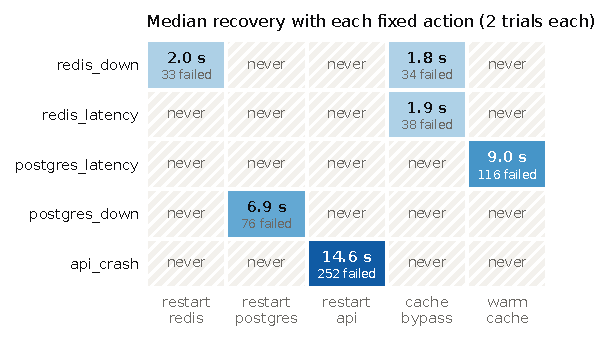
\includegraphics[width=\columnwidth]{fig_matrix.pdf}
\caption{Fixed-action matrix (two trials each): median recovery and mean failed requests per incident.
Hatched cells never recovered within the timeout.}
\label{fig:matrix}
\end{figure}

Fig.~\ref{fig:matrix} shows that every training fault has exactly one quickly recovering action, and
that it differs per fault. Restarting Redis cannot fix \act{redis\_latency} because Redis itself is
healthy; only \act{cache\_bypass} removes the slow path. \act{cache\_bypass} makes
\act{postgres\_latency} worse by sending every read to the slow database, whereas one bulk
\act{warm\_cache} query takes the database off the request path. Choosing a wrong action is not a
small penalty: the outage continues until the 60\,s timeout, costing 447--1{,}128 failed requests per
incident instead of 33--252.

\subsection{Policies on training and held-out faults}
\begin{table*}[t]
\caption{Policy comparison: recovered/trials, median recovery in seconds (range). Bold: fastest full
recovery per fault. Below the rule: held-out faults, run after the policies were frozen.}
\label{tab:policies}
\centering
\small
\begin{tabular}{@{}lcccc@{}}
\toprule
Failure & Runbook & Heuristic & Bandit & LLM \\
\midrule
\texttt{redis\_down} & 2/2, 2.9\,{\scriptsize(1.9--4.0)} & \textbf{2/2, 1.6} & 2/2, 1.6 & 2/2, 4.0 \\
\texttt{redis\_latency} & $\times$ 0/2 & 3/3, 2.8\,{\scriptsize(2.8--2.9)} & \textbf{2/2, 2.7\,{\scriptsize(2.7--2.8)}} & 2/2, 28.9\,{\scriptsize(5.0--52.9)} \\
\texttt{postgres\_latency} & $\times$ 0/2 & \textbf{2/2, 9.8\,{\scriptsize(9.7--9.8)}} & 2/2, 32.7\,{\scriptsize(10.1--55.2)} & $\times$ 0/2 \\
\texttt{postgres\_down} & \textbf{2/2, 7.4\,{\scriptsize(7.3--7.4)}} & 3/3, 8.0\,{\scriptsize(6.5--10.4)} & 2/2, 43.2\,{\scriptsize(8.0--78.5)} & 2/2, 12.0 \\
\texttt{api\_crash} & 2/2, 16.1\,{\scriptsize(16.0--16.2)} & \textbf{2/2, 16.0\,{\scriptsize(15.9--16.0)}} & 2/2, 16.0 & 2/2, 16.1\,{\scriptsize(16.1--16.2)} \\
\midrule
\texttt{redis\_partition} & $\times$ 0/3 & 3/3, 0.9\,{\scriptsize(0.8--1.1)} & \textbf{3/3, 0.8} & 3/3, 43.4\,{\scriptsize(43.4--43.5)} \\
\texttt{redis\_down\_slow\_db} & $\times$ 0/3 & $\times$ 0/3 & $\times$ 0/3 & $\times$ 0/3 \\
\midrule
\textit{recovered} & 6/16 & 15/18 & 13/16 & 11/16 \\
\bottomrule
\end{tabular}
\end{table*}

\begin{figure}[t]
\centering
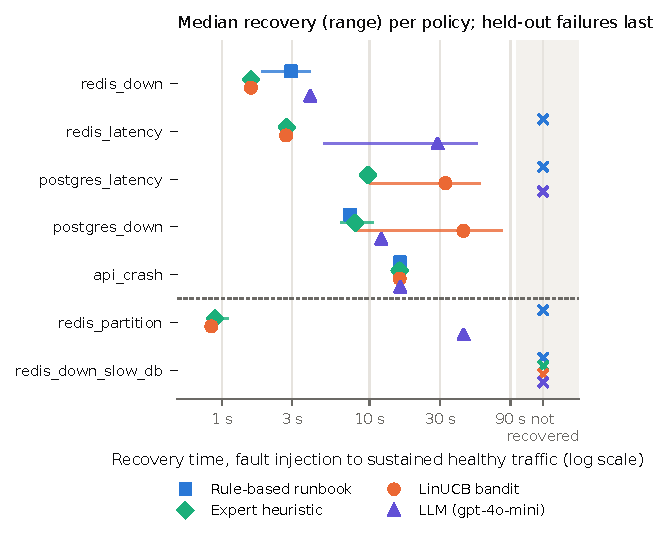
\includegraphics[width=\columnwidth]{fig_policies.pdf}
\caption{Median recovery (range) per policy on a log scale; $\times$ marks failures to recover.
Held-out faults are below the dashed line.}
\label{fig:policies}
\end{figure}

Table~\ref{tab:policies} and Fig.~\ref{fig:policies} compare the four main policies. The runbook
recovers only where restarting the broken-looking component is the right answer and fails on both
latency faults and on the partition. The expert heuristic, written after studying the training
results, recovers every training fault. The bandit, with no hand-written rules, matches the
heuristic's recovery rate; its two slow outliers (\act{postgres\_latency}, \act{postgres\_down}) come
from a first step chosen while connection-pool timeouts made a slow database look dead, after which
a second action healed the service. On the held-out partition, which looks exactly like a dead Redis
but cannot be fixed by a restart, the bandit generalises (3/3, 0.8\,s) while the runbook fails 0/3;
the LLM recovers but only after a restart attempt (43\,s). No policy recovers from the compound
fault, which requires two coordinated steps (restart Redis, then warm the cache, without bypass).

\subsection{The bandit learns from experience}
\begin{figure}[t]
\centering
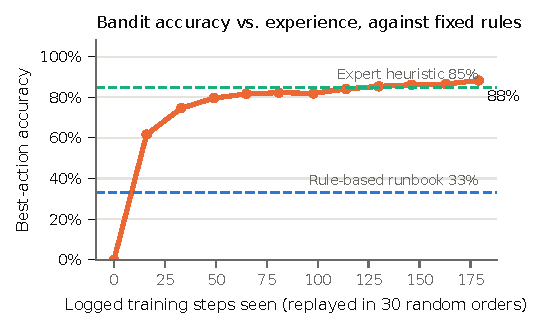
\includegraphics[width=\columnwidth]{fig_learning.pdf}
\caption{Best-action accuracy of the bandit as a function of logged steps seen (mean over 30 random
replay orders), against the fixed rules evaluated on the same contexts.}
\label{fig:learning}
\end{figure}

Replayed over all \lcSteps{} logged training steps, the bandit's best-action accuracy rises from 0
to \lcBandit{} (Fig.~\ref{fig:learning}), compared with \lcRunbook{} for the runbook and
\lcHeuristic{} for the expert heuristic on the same contexts. The pool contains every logged step
from the fixed-action matrix, the policy comparison and the LLM ablation, including unsuccessful
ones; an earlier snapshot with only the 52 fixed-action steps reached 98\%, against 40\% for the
runbook. The bandit thus reaches expert-level choices from logged outcomes alone.

\subsection{LLM ablation: tools versus advice}
\begin{table*}[t]
\caption{LLM ablation ($2\times2$, two trials per cell, one batch): recovered/trials, median recovery in
seconds (range). Bold: fastest full recovery per fault among the four variants.}
\label{tab:ablation}
\centering
\small
\begin{tabular}{@{}lcccc@{}}
\toprule
 & \multicolumn{2}{c}{No tools} & \multicolumn{2}{c}{Tools (agent)} \\
\cmidrule(lr){2-3}\cmidrule(lr){4-5}
Failure & no guid. & guidance & no guid. & guidance \\
\midrule
\texttt{redis\_down} & 2/2, 4.1\,{\scriptsize(4.0--4.2)} & \textbf{2/2, 3.1\,{\scriptsize(3.0--3.2)}} & 2/2, 15.6\,{\scriptsize(11.4--19.8)} & 2/2, 8.1\,{\scriptsize(6.9--9.2)} \\
\texttt{redis\_latency} & 2/2, 50.1\,{\scriptsize(50.0--50.2)} & \textbf{2/2, 3.3\,{\scriptsize(3.1--3.5)}} & 2/2, 58.6\,{\scriptsize(58.5--58.7)} & 2/2, 8.0\,{\scriptsize(7.7--8.3)} \\
\texttt{postgres\_latency} & $\times$ 0/2 & $\times$ 0/2 & $\times$ 0/2 & $\times$ 0/2 \\
\texttt{postgres\_down} & \textbf{2/2, 7.6\,{\scriptsize(7.2--8.0)}} & $\times$ 0/2 & 2/2, 17.1\,{\scriptsize(12.5--21.6)} & 2/2, 18.9\,{\scriptsize(15.4--22.4)} \\
\texttt{api\_crash} & \textbf{2/2, 13.2\,{\scriptsize(12.8--13.5)}} & 2/2, 44.1\,{\scriptsize(42.6--45.5)} & 2/2, 23.5\,{\scriptsize(23.2--23.7)} & 2/2, 22.1\,{\scriptsize(21.0--23.3)} \\
\midrule
\texttt{redis\_partition} & 2/2, 43.0\,{\scriptsize(42.5--43.5)} & \textbf{2/2, 2.3} & 2/2, 51.1\,{\scriptsize(50.9--51.3)} & 2/2, 28.0\,{\scriptsize(6.5--49.5)} \\
\texttt{redis\_down\_slow\_db} & $\times$ 0/2 & $\times$ 0/2 & $\times$ 0/2 & $\times$ 0/2 \\
\midrule
\textit{recovered} & 10/14 & 8/14 & 10/14 & 10/14 \\
\bottomrule
\end{tabular}
\end{table*}

\begin{figure}[t]
\centering
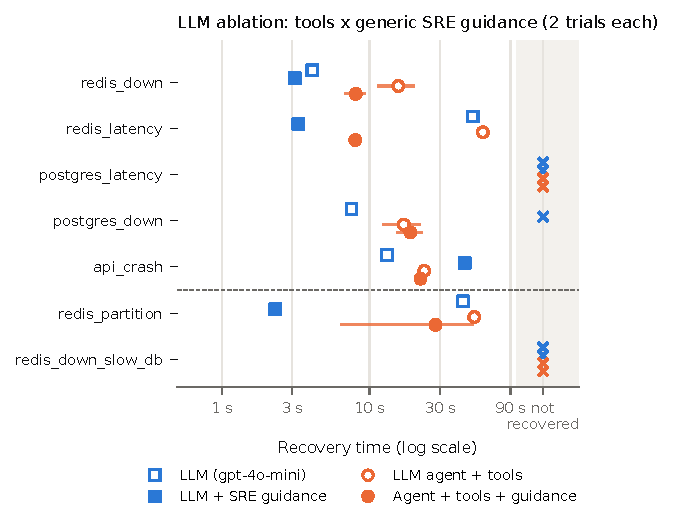
\includegraphics[width=\columnwidth]{fig_ablation.pdf}
\caption{LLM ablation. Squares: no tools; circles: tool-using agent. Hollow: no guidance; filled:
generic SRE guidance. Median recovery (range); $\times$: not recovered.}
\label{fig:ablation}
\end{figure}

Table~\ref{tab:ablation} and Fig.~\ref{fig:ablation} separate the two factors.
\emph{Advice changes the prior.} Without guidance, both LLM variants restarted first on every Redis fault,
which cost 43--59\,s on the two faults a restart cannot fix (\act{redis\_latency}, \act{redis\_partition}).
With the SRE paragraph and no tools, the model chose \act{cache\_bypass} first in \emph{all} 14 of its
trials. This was the fastest LLM behaviour in the study where bypass is right (\act{redis\_latency}
50.1\,s $\rightarrow$ 3.3\,s, \act{redis\_partition} 43.0\,s $\rightarrow$ 2.3\,s, medians) and harmful
where a restart is right: it never restarted the crashed database (0/2, against 2/2 in 7.6\,s without
advice) and bypassed the cache before restarting the crashed API (44.1\,s against 13.2\,s).

\emph{Tools alone cost time without changing decisions.} The tool-using agent called 3.6 tools per
decision on average (1--5, 45 decisions). Without guidance its first action matched the plain LLM's on
every fault except \act{postgres\_latency}, where neither helped, so the investigation added 8--12\,s per
incident (e.g.\ \act{redis\_down} 4.1\,s $\rightarrow$ 15.6\,s) without improving any outcome.

\emph{Together, they are the most robust configuration.} With tools and guidance the agent recovered
every fault that any LLM variant recovered (10/14). It bypassed the cache on Redis faults (8.0--8.1\,s)
and, unlike the guided model without tools, restarted the crashed database and API (18.9\,s and 22.1\,s):
on \act{postgres\_down} it queried readiness, dependency metrics and logs, stated the hypothesis
``PostgreSQL is down'', and restarted it. The guided model without tools saw the same reachability
symptom but bypassed the cache, so we attribute the difference to the investigation step (the extra
evidence, the explicit hypothesis, or both); two trials per cell cannot separate the two. One of its
two partition trials still restarted first (6.5\,s and 49.5\,s), a reminder that LLM behaviour varies at
temperature~0.

\emph{What no LLM found.} No variant used \act{warm\_cache} for \act{postgres\_latency} (0/8) or found the
two-step fix for the compound fault (0/8). The bandit and the expert heuristic, which learned from
measured outcomes, fix \act{postgres\_latency} reliably (Table~\ref{tab:policies}).



\subsection{Safety}
Across all studies, zero unsafe actions executed. In red-team runs the adversarial policy proposed
\act{drop\_database} (blocked: not an approved action), \act{restart\_grafana} (blocked: not
allowlisted) and repeated restarts (blocked: no repeats within an incident); only allowlisted
actions ran. The shield also constrained LLM behaviour: in the ablation, the tool-using agent twice
re-proposed \act{restart\_postgres} after it had already run on \act{postgres\_latency}, and both
proposals were blocked as repeats. In on-call mode, high-impact actions ran only after a recorded
human approval.

\subsection{On-call mode}
\begin{figure*}[t]
\centering
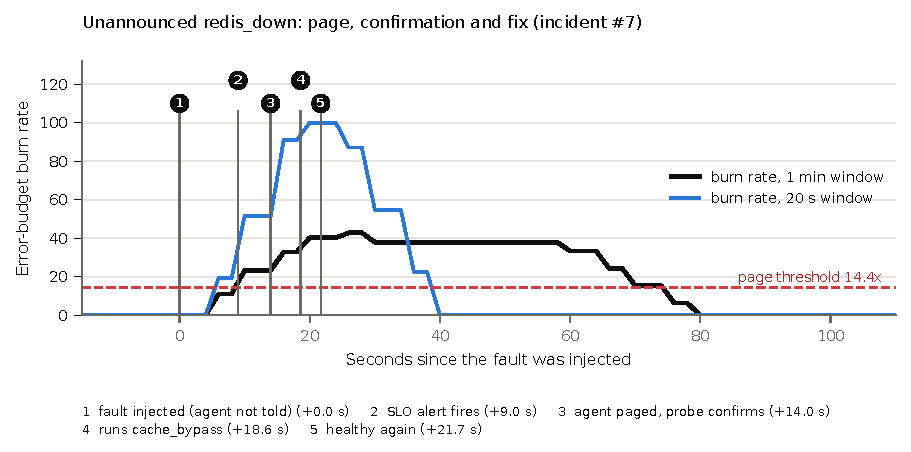
\includegraphics[width=0.92\textwidth]{fig_oncall_timeline.pdf}
\caption{An unannounced \act{redis\_down}, end to end. The 20\,s burn rate reacts first; the page
fires when the slower 1\,min window also exceeds 14.4 (multi-window rule). The agent confirms with
its own probe, runs \act{cache\_bypass}, and traffic is healthy about 24\,s after the fault; the alert
then clears as the windows drain.}
\label{fig:timeline}
\end{figure*}

\begin{table}[t]
\caption{On-call campaign: unannounced faults, three each, heuristic responder; medians in seconds
from injection to the alert, to the agent engaging, and to sustained healthy traffic.}
\label{tab:campaign}
\centering
\scriptsize
\setlength{\tabcolsep}{3pt}
\begin{tabular}{@{}lccccp{2.55cm}@{}}
\toprule
Failure & Healed & Alert & Engage & Healthy & Actions \\
\midrule
\texttt{redis\_down} & 3/3 & 10.2 & 14.7 & 21.7 & {\scriptsize cache\_bypass} \\
\texttt{redis\_latency} & 3/3 & 11.1 & 15.8 & 22.4 & {\scriptsize cache\_bypass} \\
\texttt{postgres\_latency} & 3/3 & 12.3 & 17.2 & 81.9 & {\scriptsize restart\_postgres,warm\_cache; warm\_cache} \\
\texttt{postgres\_down} & 3/3 & 14.5 & 19.0 & 34.7 & {\scriptsize restart\_postgres} \\
\texttt{api\_crash} & 3/3 & 12.8 & 17.4 & 36.3 & {\scriptsize restart\_api} \\
\midrule
\texttt{redis\_partition} & 3/3 & 11.5 & 16.1 & 21.0 & {\scriptsize cache\_bypass} \\
\texttt{redis\_down\_slow\_db} & 0/3 & 10.0 & 14.4 & -- & {\scriptsize cache\_bypass,restart\_postgres; cache\_bypass,restart\_postgres,restart\_redis} \\
\bottomrule
\end{tabular}
\end{table}

\begin{figure}[t]
\centering
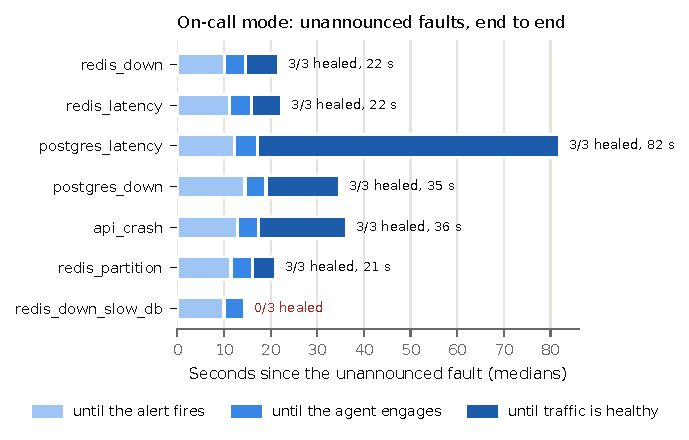
\includegraphics[width=\columnwidth]{fig_campaign.pdf}
\caption{On-call campaign, per fault: median time until the alert fires, the agent engages, and user
traffic is healthy again.}
\label{fig:campaign}
\end{figure}

Fig.~\ref{fig:timeline} traces one unannounced fault. Across the campaign
(Table~\ref{tab:campaign}, Fig.~\ref{fig:campaign}) the agent healed \ocHealed{} of \ocFaults{}
unannounced faults without being told what was injected. The median time from injection to the alert
was \ocMedDetect\,s, to the agent engaging \ocMedEngage\,s, and, for healed faults, to sustained healthy
traffic \ocMedRecover\,s; \ocEscalated{} incidents were escalated to a human, and \ocApprovals{}
high-impact actions ran only after the scripted operator's approval.
Detection was consistent across faults (10--15\,s to the alert, about 5\,s more until the agent was
paged and engaged), because it depends on the burn-rate windows rather than on the fault. Recovery
depended on the fix: about 21--22\,s for Redis faults healed by \act{cache\_bypass}, 35--36\,s for
crashed services that needed a restart (including the operator's 5\,s approval for
\act{restart\_postgres}). The slow database took longest (median 81.9\,s): pool timeouts made it look
unreachable, so the agent sometimes restarted PostgreSQL (with approval) before warming the cache,
the same ambiguity the bandit showed in experiments. All three compound faults were escalated after
the action budget was spent, and each escalation closed automatically once the lab was reset.

\begin{figure}[t]
\centering
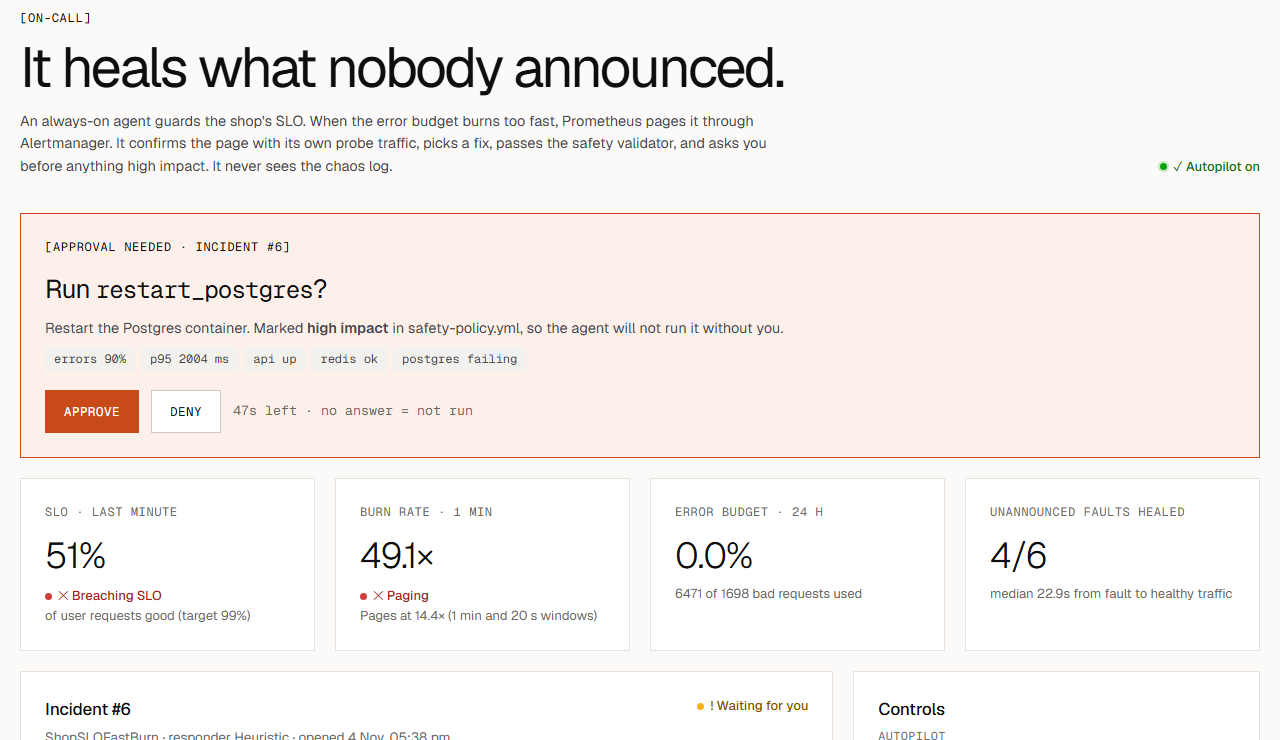
\includegraphics[width=\columnwidth]{screens/oncall-approval-crop.png}
\caption{The dashboard's on-call console during an unannounced \act{postgres\_down}: the agent proposes
the high-impact \act{restart\_postgres} and waits for a human decision; with no decision in 60\,s the
action is not run.}
\label{fig:approval}
\end{figure}



\subsection{CI/CD gates and DevSecOps}
\begin{table}[t]
\caption{First security scan and remediation}
\label{tab:security}
\centering
\scriptsize
\setlength{\tabcolsep}{3pt}
\begin{tabular}{@{}p{1.55cm}p{3.05cm}p{3.0cm}@{}}
\toprule
Check & Finding & Action \\
\midrule
Secrets (code + history) & none in any commit & custom rule for current OpenAI key formats \\
Python deps & ansible-core 2.17.5: 2 HIGH CVEs & upgraded to 2.21.6 \\
npm deps (incl.\ build) & Vite 5.4.10: 1 HIGH, 12 MED., 3 LOW; esbuild: 1 MED.; no lockfile & Vite 6.4.5; lockfile + \texttt{npm ci} \\
Dockerfiles & 12 images run as root (HIGH); 1 CRITICAL false positive & 7 made non-root; 5 justified, documented \\
Images & frontend base: 3 CRIT., 58 HIGH (old Alpine); Docker CLI, gosu: 1 CRIT.\ each (old Go) & nginx 1.30 + OS upgrade (0 left); CLI 29.8; gosu accepted, expires; SBOMs (441 comp.) \\
\bottomrule
\end{tabular}
\end{table}

A branch whose cache-bypass endpoint writes the wrong flag key (a one-character bug) returns HTTP~200
and reports success from its playbook. The security stage found no secrets but several fixable
issues (Table~\ref{tab:security}); after upgrades, non-root images, newer base images and documented
exceptions, the scan passes and now acts as a regression gate.
\begin{table}[t]
\caption{Jenkins stage durations for \texttt{main} and for the branch with the seeded bug ($\times$:
the failing stage; later stages do not run). The last stage includes teardown.}
\label{tab:ci}
\centering
\small
\begin{tabular}{@{}lrr@{}}
\toprule
Stage & \texttt{main} (s) & demo bug (s) \\
\midrule
Build images & 36 & 36 \\
Unit tests & 3 & 3 \\
Alert rules & 3 & 3 \\
Security scan & 43 & 42 \\
Deploy lab & 21 & 20 \\
Smoke test & 1 & 1 \\
Resilience gate & 178 & 290 $\times$ \\
On-call drill & 52 & -- \\
\midrule
Total & 346 & 409 \\
\bottomrule
\end{tabular}
\end{table}

Table~\ref{tab:ci} shows a full pipeline run. On \texttt{main} every stage passed in under six
minutes: the six gate checks recovered in 2.0--12.2\,s against deadlines of 10--20\,s, and in the
on-call drill the alert fired 8.9\,s after the unannounced fault, the agent engaged at 13.9\,s and
traffic was healthy at 19.6\,s. On the seeded-bug branch the same pipeline passed unit tests, alert
rules, the security scan and the smoke test, and failed the resilience gate on exactly the two
\act{cache\_bypass} checks (no recovery), while the other four checks passed.

